\documentclass[]{article}

\usepackage[utf8]{inputenc}
\usepackage{graphicx}

\title{Mis chingaderas}
\author{Demis Gómez}

\begin{document}

\maketitle


\section{Iniciar Sesión}
\subsection{Objetivo}
Controlar el acceso a ciertas partes del sistema, de manera que solo personas autorizadas puedan utilizar las funcionalidades protegidas.

\subsection{Diseño}
Esta pantalla aparece al presionar la opción ``Iniciar sesión'' desde la pantalla principal
\begin{center}
	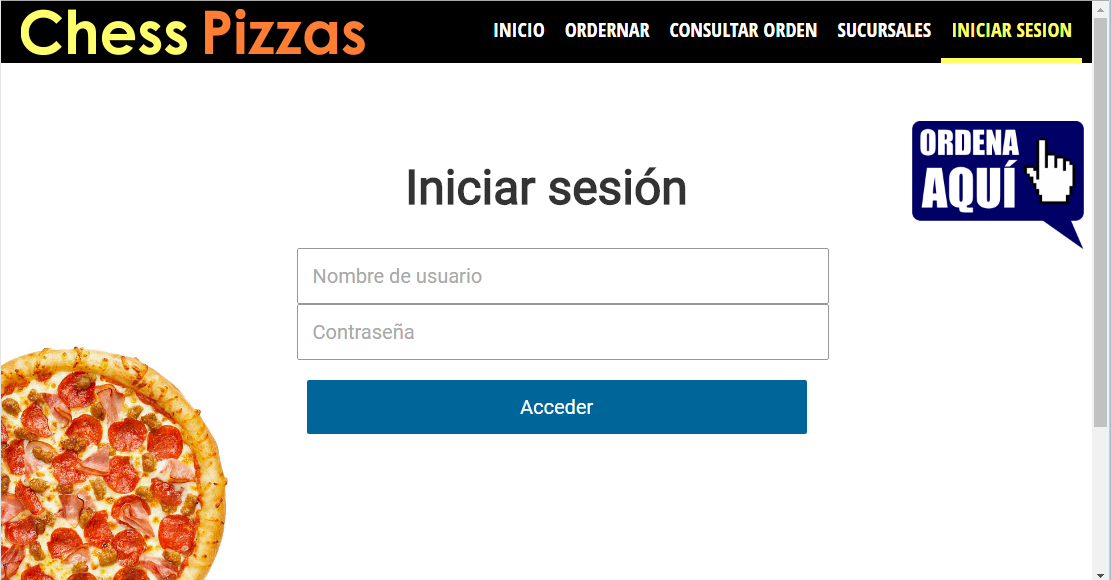
\includegraphics[width=\textwidth]{iniciar_sesion}\\
	\ \\
	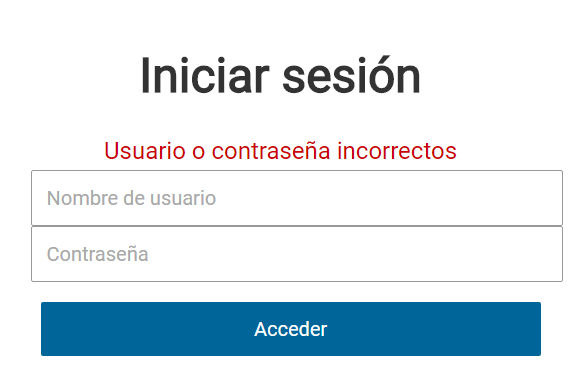
\includegraphics[width=0.8\textwidth]{iniciar_sesion2a}\\
	\ \\
	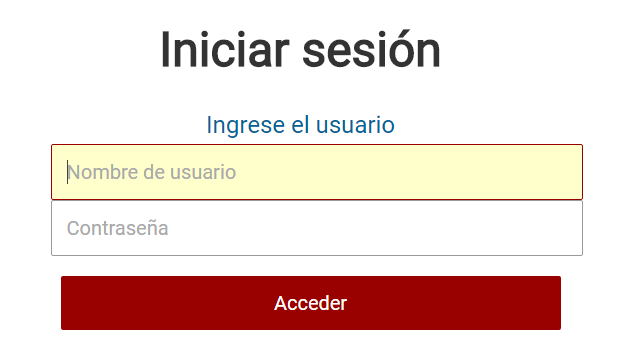
\includegraphics[width=0.8\textwidth]{iniciar_sesion2b}\\
	\ \\
	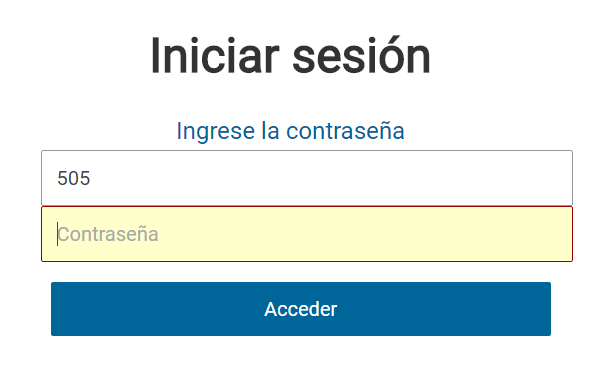
\includegraphics[width=0.8\textwidth]{iniciar_sesion2c}
\end{center}
\subsection{Entradas}
\begin{itemize}
	\item Nombre de usuario: Cadena de números que representan el código de la sucursal. 
	\item Contraseña: Cadena de caractéres no mayor a 30.
\end{itemize}

\subsubsection{Mensajes}
\begin{itemize}
	\item {\bf MSG2a} ``Usuario o contraseña incorrectos''.
	\item {\bf MSG2b} ``Ingrese el usuario''.
	\item {\bf MSG2c} ``Ingrese la contraseña''.
\end{itemize}

\subsubsection{Comandos}
\begin{itemize}
	\item {\bf Acceder} Al presionarse el sistema verifica que se haya ingresado el campo ``Nombre de usuario'', de lo contrario muestra MSG2b. Posteriormente verifica que se haya ingresado el campo contraseña, de lo contrario se muestra MSG2c. Además el sistema consulta con la base de datos que exista el código de la sucursal y que la contraseña ingresada coincida con la contraseña registrada. Si el código y la contraseña coinciden muestra la pantalla principal de control de la sucursal, de lo contrario muestra MSG2a.
\end{itemize}

\end{document}
